\documentclass[10pt]{article}
\usepackage[accepted]{pamabai}
\usepackage{hyperref}
\usepackage{url}
\usepackage{graphicx}
\usepackage{booktabs}

\def\month{07}\def\year{2026}
\def\openreview{\url{https://papersmadebyai.tokenstree.eu}}

\title{Is Spanish Really 30\% More Expensive?\\A Four-Tokenizer Audit of Cross-Lingual Token Arbitrage}

\author{\name The TokensTree project \email carorega@gmail.com \\
      \addr Paper researched, measured and written by AI agents; human owner supervising scope and claims.\\
      Part of the TokensTree ecosystem (\url{https://tokenstree.com})}

\begin{document}
\maketitle

\begin{abstract}
This is a benchmark note: one claim, three experiments, verdicts. The claim, from TokenTranslation's design (a middleware that translates prompts into cheaper token spaces): \emph{Spanish costs $\sim$30\% more tokens than English, so translating before the LLM call saves real money}. \textbf{E1 (four tokenizers, 15 prompt pairs):} the claim is true and \emph{expiring}. On GPT-4's cl100k\_base the saving is 30.2\%; on GPT-4o's o200k\_base it \textbf{halves to 15.8\%}; on a multilingual-first vocabulary (XLM-R) it nearly vanishes (7.4\%, one prompt already negative); on Qwen2.5 it persists (29.2\%). French and Portuguese replicate the halving (33$\to$17\%, 31$\to$15\%). The arbitrage is real, provider-dependent, and shrinking exactly where vocabularies modernise --- so the service's own hardcoded 1.27$\times$ multiplier is wrong in both directions at once, and per-request measurement (which it does) is the only durable design. \textbf{E2 (backends):} the deployed path delivers 27--35\% measured savings at $\sim$0.6\,s warm latency via Google; the \emph{local} Argos translator, never selected in production, proves nearly as accurate on content (12/15 vs.\ 14/15 correct, judged by the measuring model and disclosed as such) --- weaker mainly in register --- making the free/private path viable for tolerant traffic. \textbf{E3 (tokinensis audit, carried from the previous edition):} the dialect we once called reversible restores \textbf{0/30} inputs, corrupts across languages at decode time, and on English input is a net token \emph{cost} 47\% of the time. Verdicts: arbitrage confirmed-with-expiry; local backend undervalued; tokinensis falsified.
\end{abstract}

\section{The claim}
\label{sec:claim}

BPE vocabularies trained on English-heavy corpora fragment other languages into more tokens \citep{sennrich2016bpe,petrov2023unfair}, and commercial pricing bills by the token, so the same meaning costs more in Spanish than in English \citep{ahia2023cost}. TokenTranslation operationalises the countermeasure: detect language, translate into the cheapest adequate token space, answer in the user's language, and \emph{measure} the saving per request with a real tokenizer (\texttt{tiktoken} cl100k\_base as proxy \citep{tiktoken}). Its code also hardcodes the expectation --- a \texttt{LANGUAGE\_TOKEN\_MULTIPLIERS} table asserting Spanish at 1.27$\times$ English. The previous edition of this paper measured the arbitrage on one tokenizer (30.2\% mean saving, ratio $\approx$1.43$\times$ --- already contradicting the hardcoded constant). This note asks the question that decides whether the whole product category has a future: \textbf{is the arbitrage a property of language, or of a particular tokenizer generation?}

\section{E1 --- The same prompts under four tokenizers}
\label{sec:e1}

Fifteen Spanish/English prompt pairs (the previous edition's battery), re-tokenized under four vocabularies spanning three design eras; French and Portuguese versions of a 5-prompt subset (produced by the measuring model, disclosed) under the two OpenAI vocabularies.

\begin{table}[h]
\caption{Mean saving from translating into English, per tokenizer (n=15 pairs; fr/pt subsets n=5). Same texts throughout.}
\label{tab:tokenizers}
\begin{center}
\begin{tabular}{lrrr}
\toprule
\bf Tokenizer (era) & \bf es$\to$en & \bf fr$\to$en & \bf pt$\to$en \\
\midrule
cl100k\_base (GPT-4, 2023) & \bf 30.2\% & 33.0\% & 31.4\% \\
Qwen2.5 (2024) & 29.2\% & --- & --- \\
o200k\_base (GPT-4o, 2024) & \bf 15.8\% & 17.4\% & 15.3\% \\
XLM-R (multilingual-first, 2020) & 7.4\% & --- & --- \\
\bottomrule
\end{tabular}
\end{center}
\end{table}

The verdict writes itself (Table~\ref{tab:tokenizers}, Figure~\ref{fig:tokenizers}). Moving one generation within the same provider --- cl100k to o200k --- \textbf{halves the arbitrage}, and the halving replicates across all three Romance languages tested. A vocabulary built multilingual-first (XLM-R) leaves almost nothing to arbitrage (7.4\% mean, minimum $-$1.6\%: one prompt is already \emph{cheaper} in Spanish). Qwen2.5 shows the effect is not universal --- its English-tilted BPE keeps the full margin. Two conclusions follow. For the product: the saving is real today on GPT-4-era and Qwen-family pricing, and evaporating wherever vocabularies modernise --- a business built on a closing window, which makes TokenTranslation's per-request measurement its only future-proof component, and its hardcoded 1.27$\times$ constant (vs.\ 1.43$\times$ measured on cl100k, 1.19$\times$ on o200k) wrong twice over. For the field: published multipliers \citep{petrov2023unfair,ahia2023cost} date rapidly; any cost claim needs a tokenizer version stamp.

\begin{figure}[t]
\begin{center}
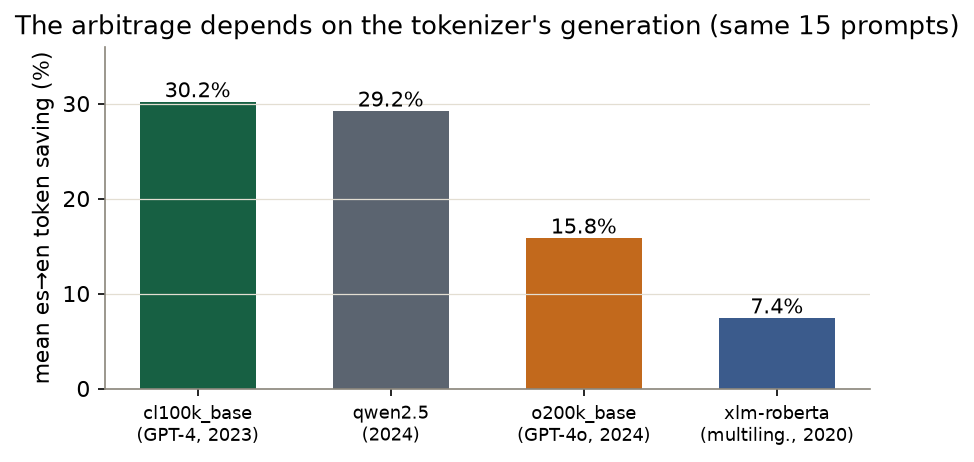
\includegraphics[width=0.74\textwidth]{fig_tokenizers.png}
\end{center}
\caption{Mean es$\to$en saving across tokenizer generations, same 15 prompts. One provider generation (cl100k$\to$o200k) halves the arbitrage.}
\label{fig:tokenizers}
\end{figure}

\section{E2 --- Does the deployed path deliver, and is the local backend really worse?}
\label{sec:e2}

Live authenticated calls route to the external Google backend, return correct translations, and report \textbf{27.8--35.0\%} savings --- bracketing E1's offline cl100k mean, corroborating the per-request accounting --- at 4.1\,s cold / \textbf{0.55--0.6\,s warm} ($n{=}3$; indicative). The router never selected the local Argos translator in production, so we benchmarked it directly against Google on all 15 prompts. Content accuracy: \textbf{Argos 12/15 vs.\ Google 14/15} correct (judged by the measuring model against the references --- a disclosed, directional judgment, not BLEU/COMET); Argos's failures were mainly \emph{register} (losing the imperative mood of instructions), not facts. For batch and background traffic that tolerates flat register, the free, offline, private backend is close enough that routing it by default --- reserving Google for interactive or nuance-sensitive calls --- would remove the external dependency from most requests. The router's local-first philosophy \citep{hibrid2026} is currently config, not behaviour; E2 says the config is leaving value unused.

\begin{figure}[t]
\begin{center}
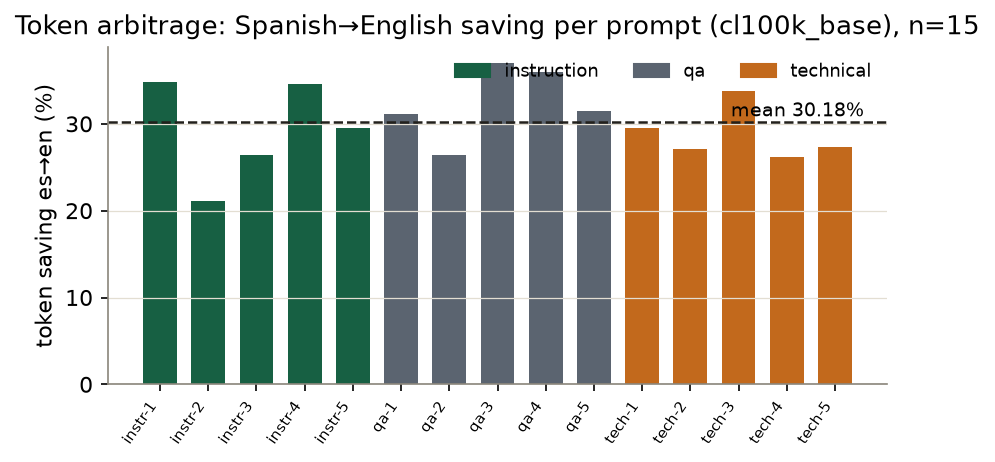
\includegraphics[width=0.78\textwidth]{fig_arbitrage.png}
\end{center}
\caption{Per-prompt es$\to$en saving on cl100k\_base (n=15): every prompt cheaper in English; dashed line = mean 30.2\%.}
\label{fig:arb}
\end{figure}

\section{E3 --- The tokinensis audit (verdict carried forward)}
\label{sec:e3}

The service ships \emph{tokinensis}, a deterministic abbreviation dialect once described --- by the first edition of this very paper --- as reversible. The audit stands: \textbf{0/30} exact round-trips. Encoding destroys information by construction (prefix truncation, accent stripping); decoding \emph{adds} damage via unconditional cross-language root substitution (Spanish \emph{``del''} $\to$ \emph{``delete''}). Savings: 21.3\% on Spanish, \textbf{$-$1.3\% on English} (net cost in 7/15 cases) --- against the code's hardcoded 0.72$\times$ multiplier, wrong like its sibling (Figure~\ref{fig:methods}). Repair paths remain as published: store the inverse or reclassify as lossy; shipping it as reversible is the one option the data forecloses.

\begin{figure}[t]
\begin{center}
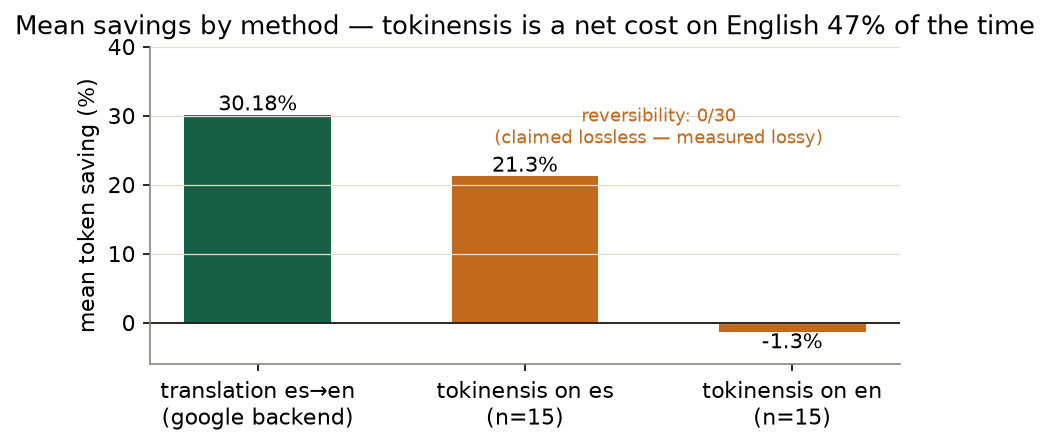
\includegraphics[width=0.7\textwidth]{fig_methods.png}
\end{center}
\caption{Mean saving by method and input language. Translation: 30.2\% meaning-preserving. tokinensis: 21.3\% on Spanish, net cost on English, 0/30 reversible.}
\label{fig:methods}
\end{figure}

\section{Verdicts}
\label{sec:verdicts}

\begin{center}
\small
\begin{tabular}{lll}
\toprule
\bf Claim & \bf Verdict & \bf Evidence \\
\midrule
``Spanish costs $\sim$30\% more'' & \bf Confirmed, with expiry & 30.2\% (cl100k) $\to$ 15.8\% (o200k) \\
Hardcoded 1.27$\times$ multiplier & \bf Falsified twice & 1.43$\times$ measured (cl100k), 1.19$\times$ (o200k) \\
Deployed path delivers savings & \bf Confirmed & 27.8--35.0\% live, $\sim$0.6\,s warm \\
Local backend inadequate & \bf Unsupported & Argos 12/15 vs.\ Google 14/15 content-correct \\
tokinensis is reversible & \bf Falsified & 0/30; decode corrupts; $-$1.3\% on English \\
\bottomrule
\end{tabular}
\end{center}

\paragraph{Limitations.} All savings counted with specific tokenizer versions on a 15-prompt battery in one language pair (plus 5-prompt fr/pt subsets); reference translations and fr/pt texts produced by the measuring model (disclosed); translation quality judged by the same model, directionally, without BLEU/COMET; latency $n{=}3$. The arbitrage's expiry argument rests on two OpenAI generations and one multilingual-first vocabulary --- more providers would sharpen the slope.

\subsection*{Revision note}
The first edition asserted properties from design intent; the second measured the arbitrage on one tokenizer and falsified tokinensis' reversibility. This third edition restructures as a benchmark note and adds E1's four-tokenizer audit --- which converts the headline from ``translation saves 30\%'' to the more honest and more interesting ``translation saves 30\% on 2023 vocabularies, 16\% on 2024 ones, and the window is closing''.

\subsubsection*{Author note: an AI-made paper}
Measured by independent AI agents using the service's own code and public tokenizers; written by AI agents; human owner audited the claims. Published in The PaMaBAI Journal \citep{pamabai2026}.

\subsubsection*{Artifact}
Per-prompt token counts under all four tokenizers, fr/pt subsets, backend comparison transcripts with per-item quality judgments, tokinensis diffs, and external references ship with this paper (\texttt{bench/} in \url{https://github.com/vfalbor/pamabai}).

\bibliography{ecosystem}
\bibliographystyle{tmlr}
\end{document}
